 \subsection[Dist Sole]{DIstanza dal Sole}
        \begin{frame}{Traiettorie}
            \begin{columns}
                \column{.6\textwidth}
                    %\centering
                    Nel tempo il sistema trasla $\Rightarrow$ I pianeti non compiono orbite chiuse.\\
                    Per valutare la stabilità del sistema è necessario monitorare l'andamento della distanza di ogni pianeta dal Sole, non ddall'origine del sistema di riferimento.
                    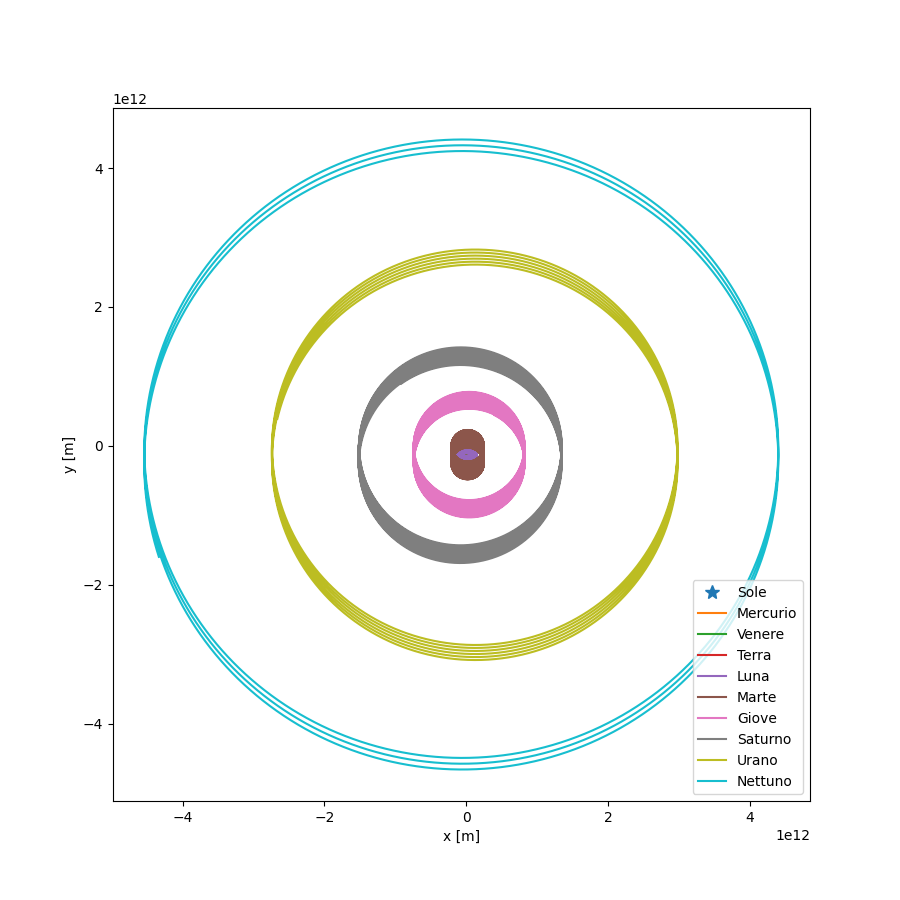
\includegraphics[width=.9\textwidth]{5_distanza/sistema_orbite.png}
                    \label{cfr::orb} 
                \column{.4\textwidth}
                    \centering
                    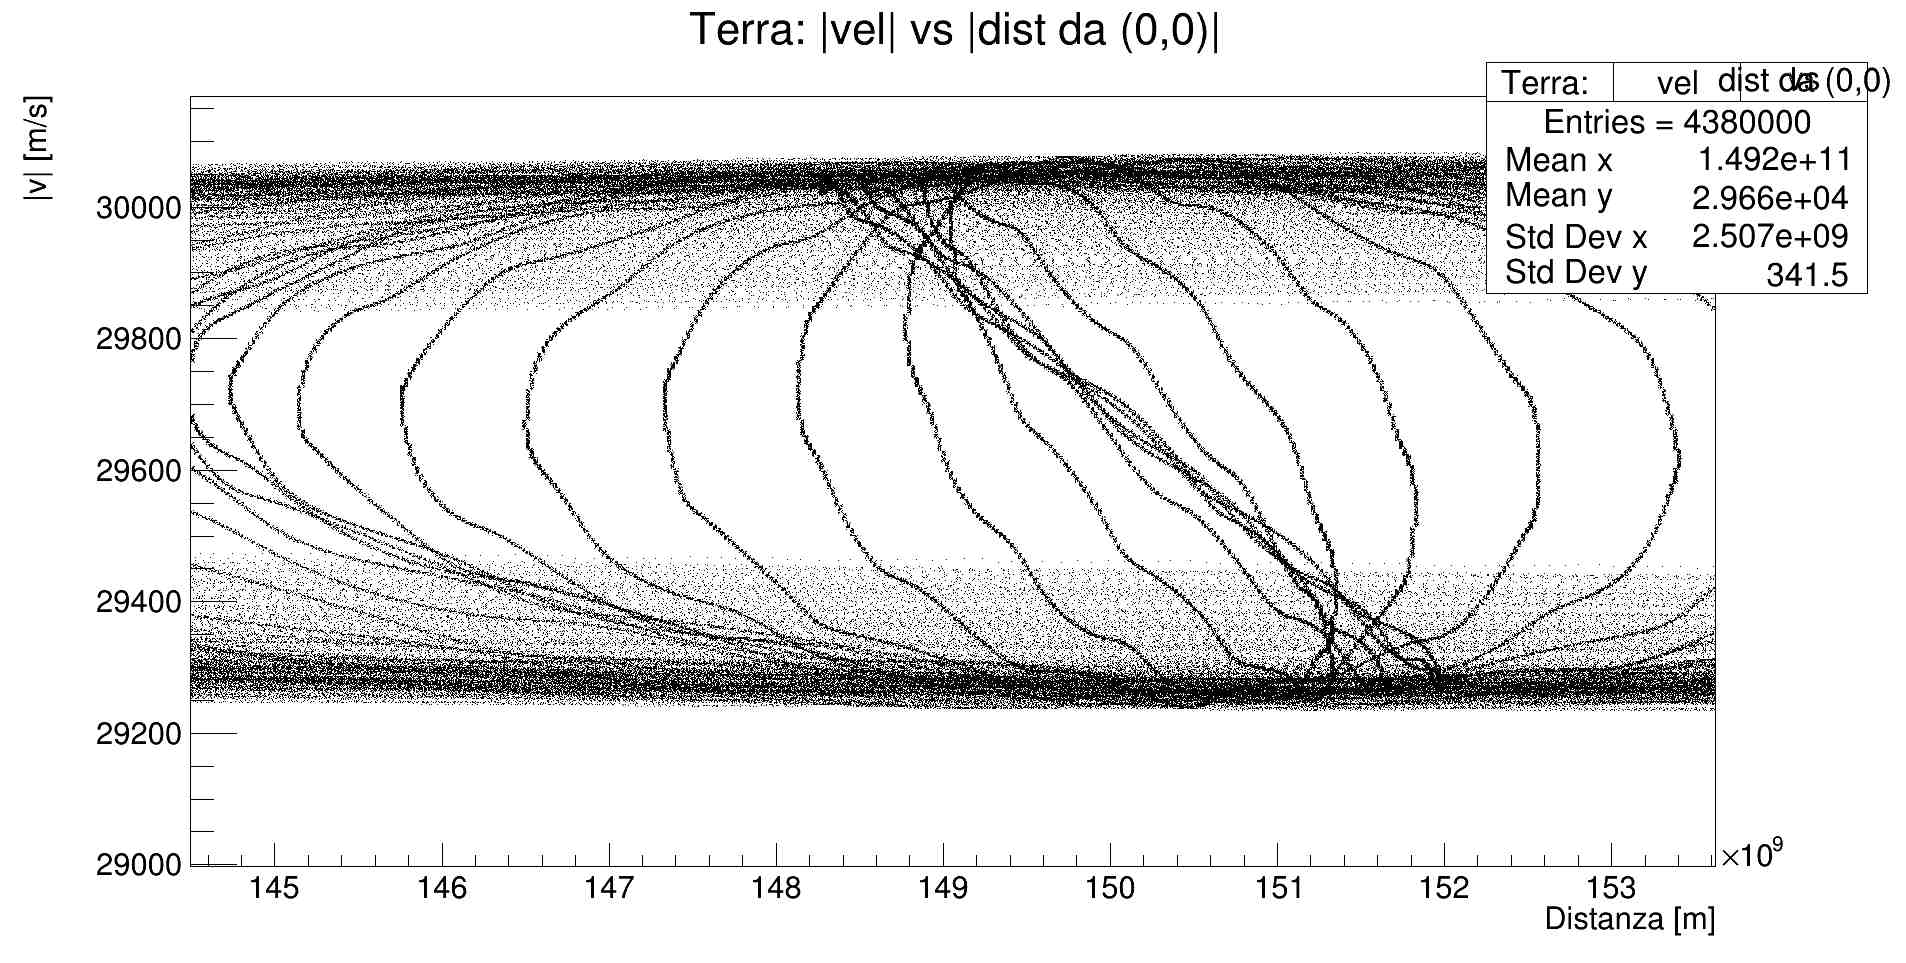
\includegraphics[width=.9\textwidth, height=3.75cm]{5_distanza/ter_vd_errato.jpg}
                    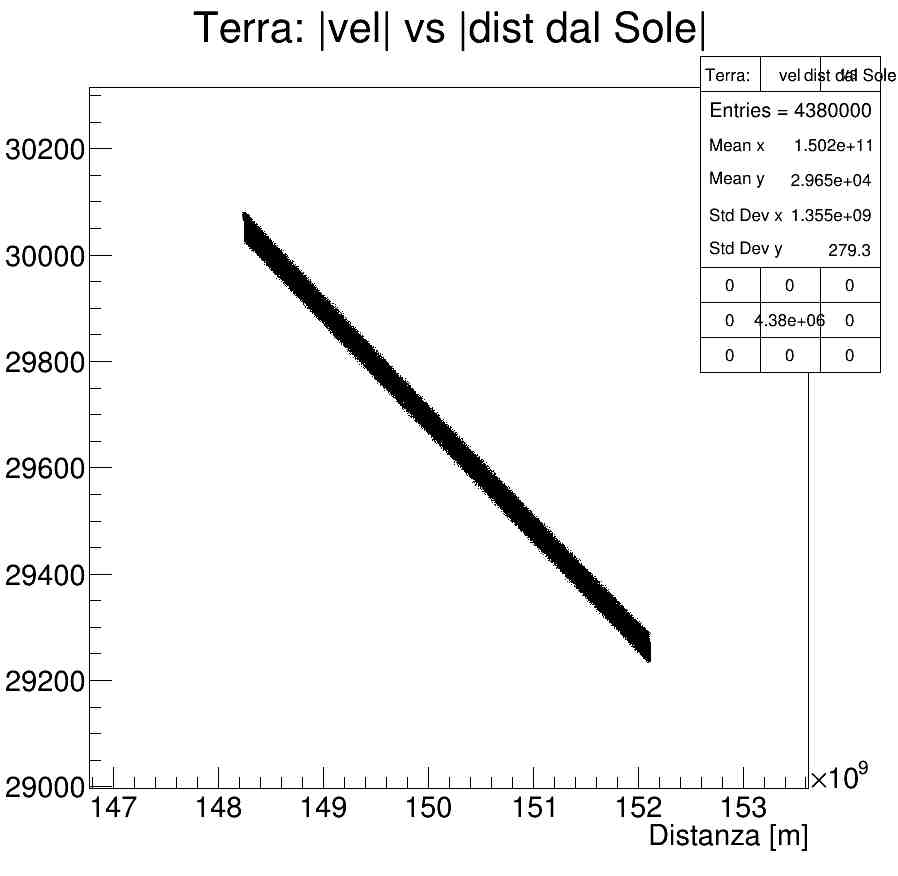
\includegraphics[width=.9\textwidth]{5_distanza/terra_vdds_luna.jpg}
            \end{columns}
        \end{frame}
        
        \begin{frame}{Istogramma Velocità - distanza dal Sole}
            \begin{columns}
                \column{.5\textwidth}
                    \centering
                    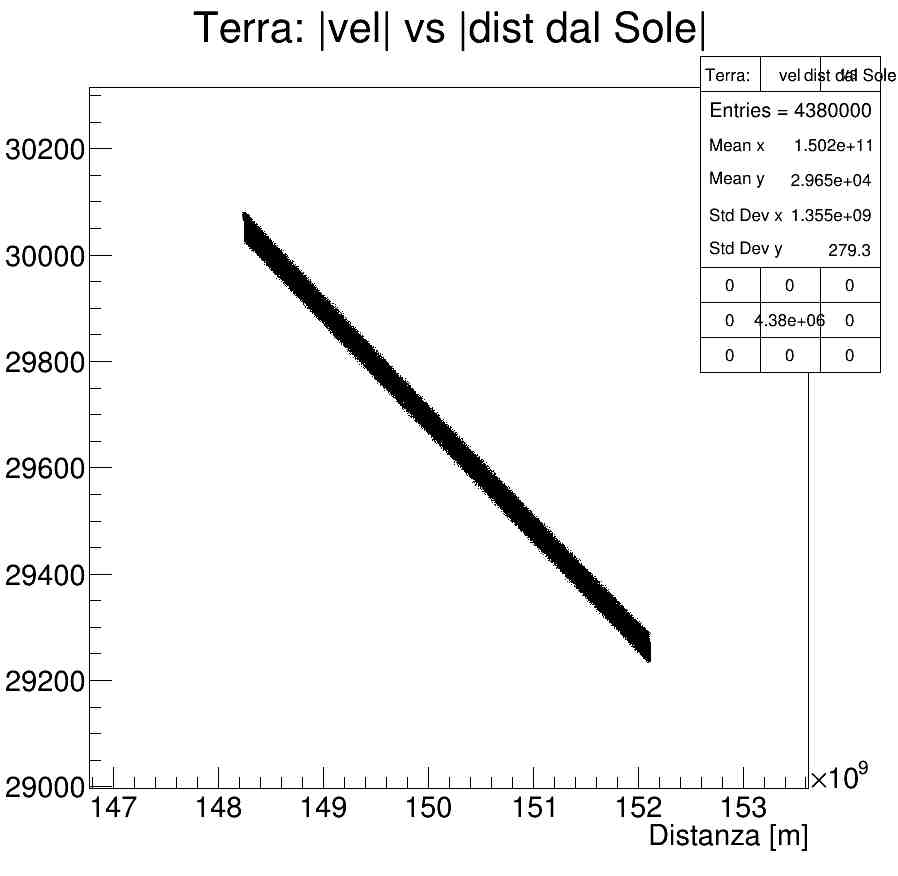
\includegraphics[width=.9\textwidth]{5_distanza/terra_vdds_luna.jpg}
                    \caption{Con la Luna}
                \column{.5\textwidth}
                    \centering
                    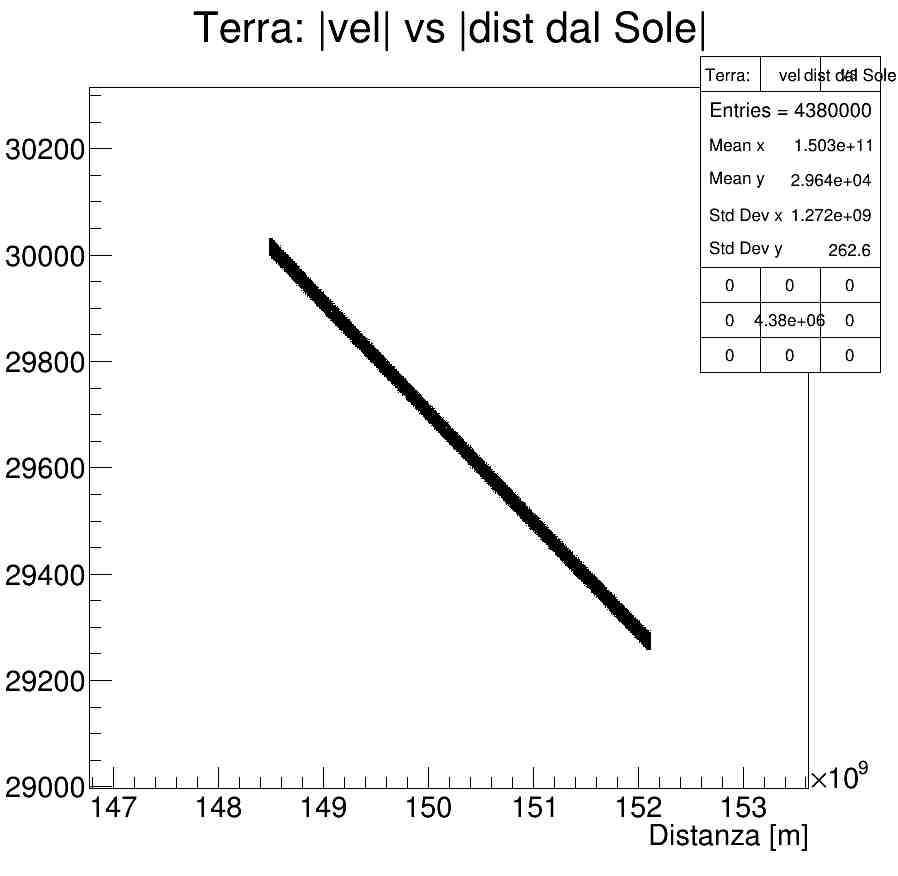
\includegraphics[width=.9\textwidth]{5_distanza/terra_vds_noluna.jpg}
                    \caption{Senza Luna}
            \end{columns}
        \end{frame}
        \begin{frame}{Istogramma Velocità - distanza dal Sole}
            \begin{columns}
                \column{.5\textwidth}
                    \centering
                    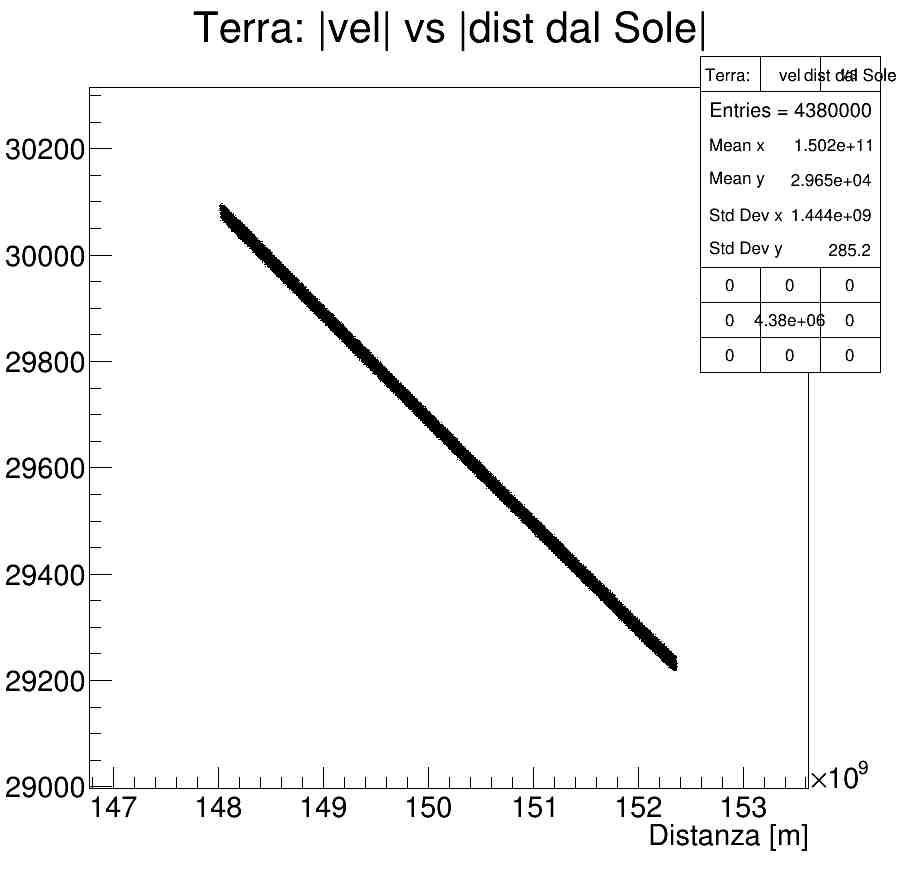
\includegraphics[width=.9\textwidth]{5_distanza/terra_vds_solefisso_luna.jpg}
                    \caption{Con il Sole fisso e la Luna}
                \column{.5\textwidth}
                    \centering
                    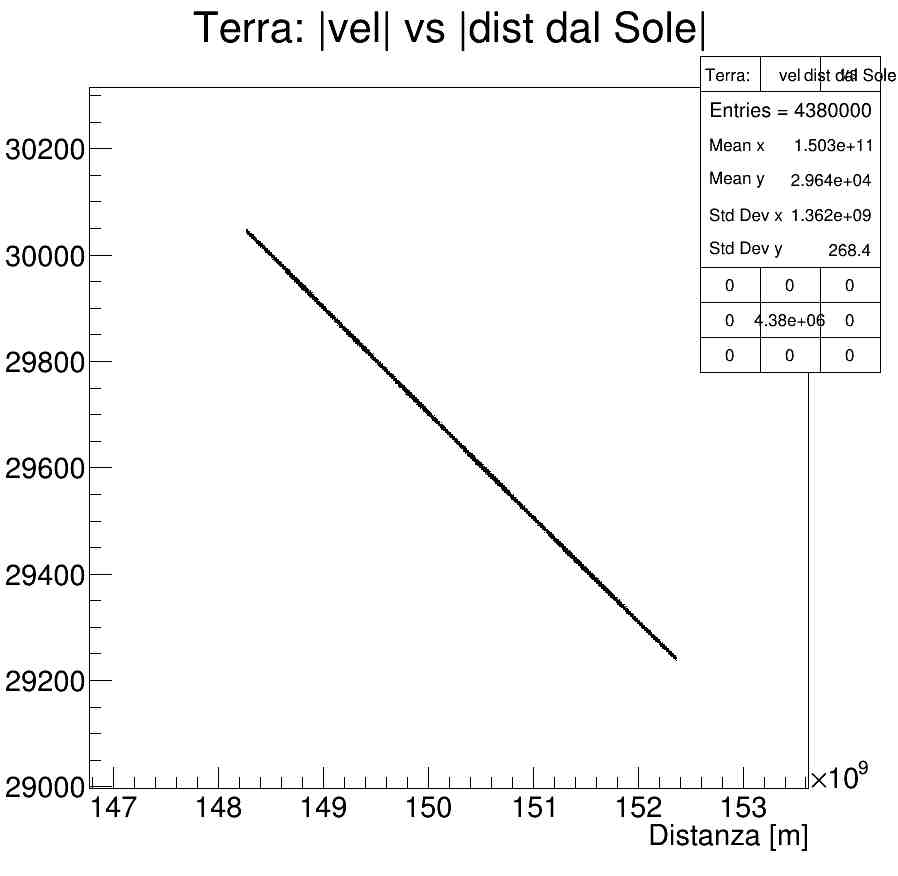
\includegraphics[width=.9\textwidth]{5_distanza/terra_vds_solefisso_noluna.jpg}
                    \caption{Con il Sole fisso e senza Luna}
            \end{columns}
        \end{frame}
        
        \begin{frame}{Distanza vs posizioni iniali}
            \begin{columns}
                \column{.35\textwidth}
                    In questo caso risultati differenti a seconda del pianeta:
                    \begin{enumerate}
                        \item Nettuno - ottimale con dati perielio
                    \end{enumerate}
                \column{.65\textwidth}
                    \centering
                    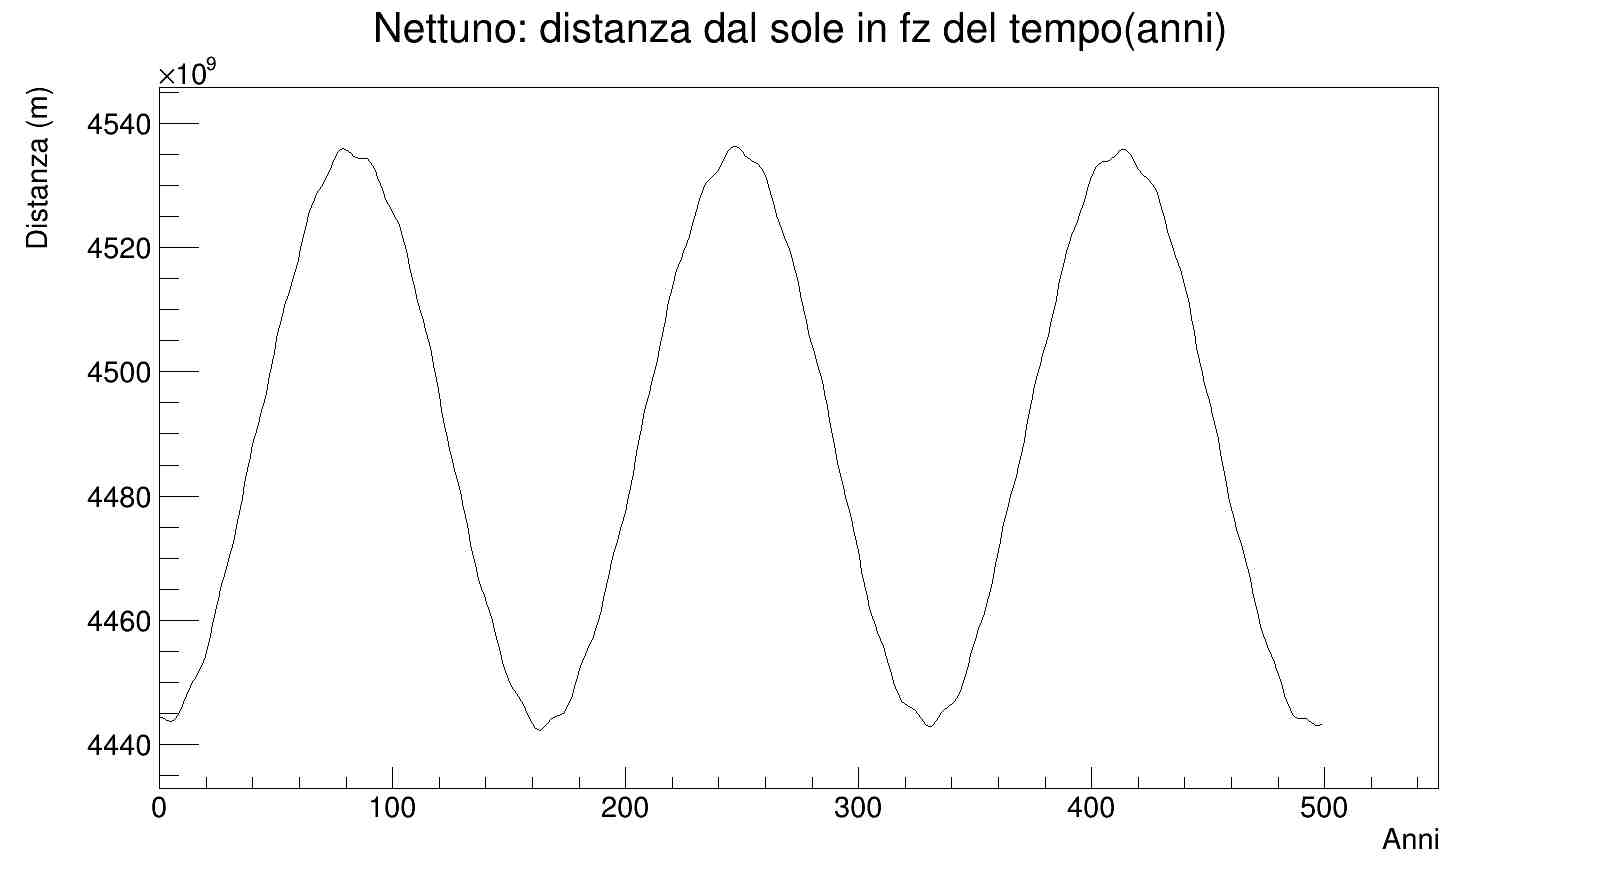
\includegraphics[width=\textwidth]{5_distanza/Net_epri_500.jpg}
                    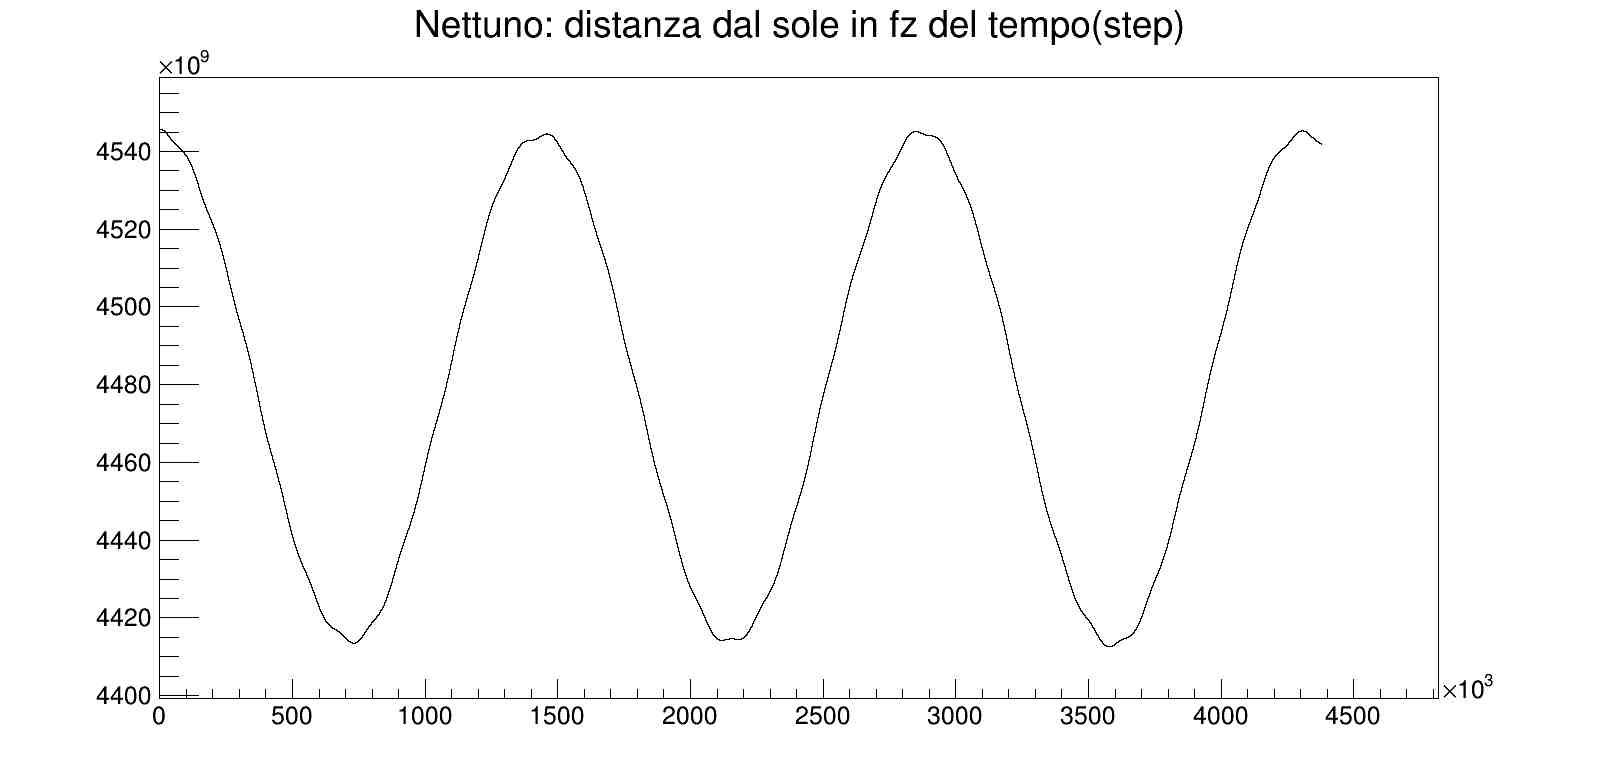
\includegraphics[width=\textwidth]{5_distanza/net_afe_500.jpg}
                    \caption{Dati perielio(in alto) e dati afelio(sotto)}
                    \label{cfr::net} 
            \end{columns}
        \end{frame}
        \begin{frame}{Distanza vs posizioni iniali}
            \begin{columns}
                \column{.35\textwidth}
                    In questo caso risultati differenti a seconda del pianeta:
                    \begin{enumerate}
                        \item Nettuno - ottimale con dati perielio
                        \item Venere - sempre leggermente fuori misura
                    \end{enumerate}
                \column{.65\textwidth}
                    \centering
                    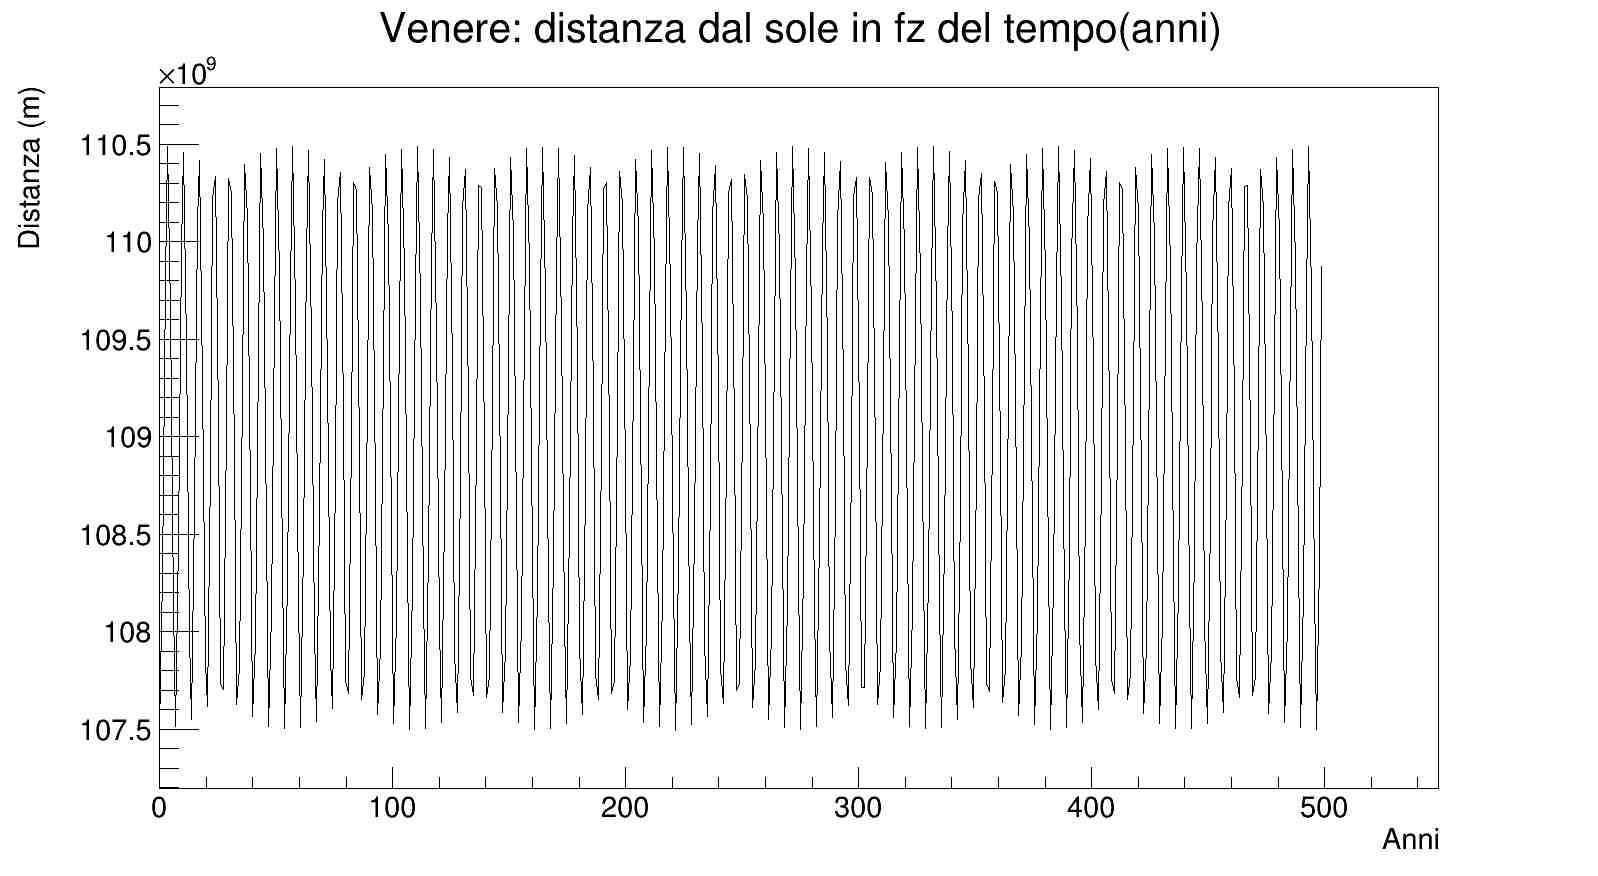
\includegraphics[width=\textwidth]{5_distanza/Ven_peri_500.jpg}
                    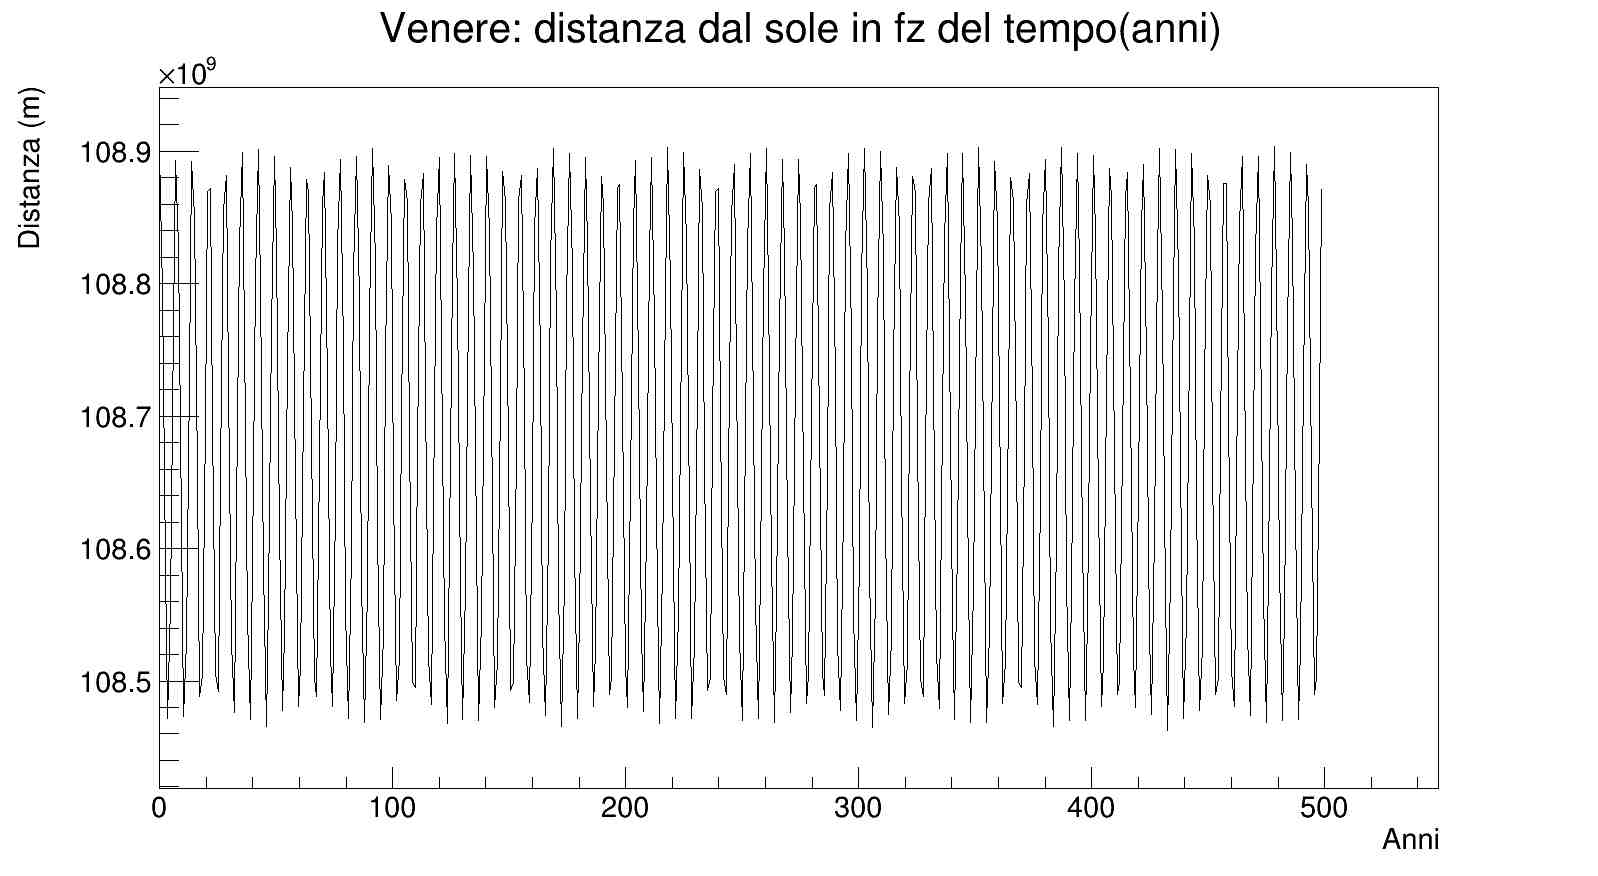
\includegraphics[width=\textwidth]{5_distanza/Ven_afe_500.jpg}
                    \caption{Dati perielio(in alto) e dati afelio(sotto)}
                    \label{cfr::ven} 
            \end{columns}
        \end{frame}
        \begin{frame}{Distanza vs posizioni iniali}
            \begin{columns}
                \column{.35\textwidth}
                    In questo caso risultati differenti a seconda del pianeta:
                    \begin{enumerate}
                        \item Nettuno - ottimale con dati perielio
                        \item Venere - sempre leggermente fuori misura
                        \item tutti errati con dati medi
                    \end{enumerate}
                \column{.65\textwidth}
                    \centering
                    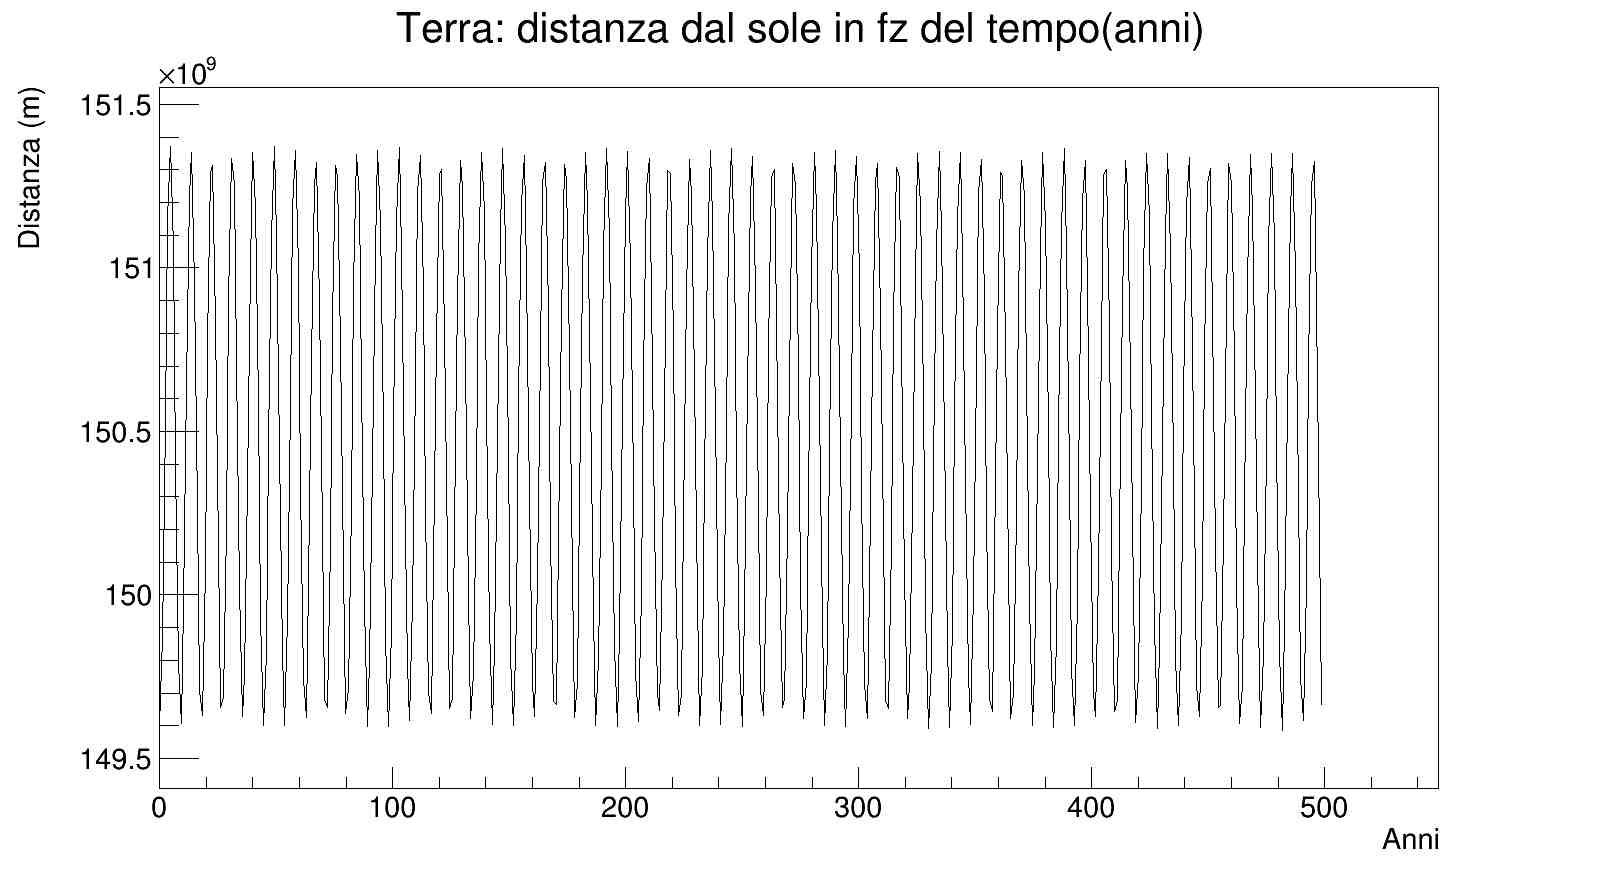
\includegraphics[width=\textwidth]{5_distanza/terra_medi.jpg}
                    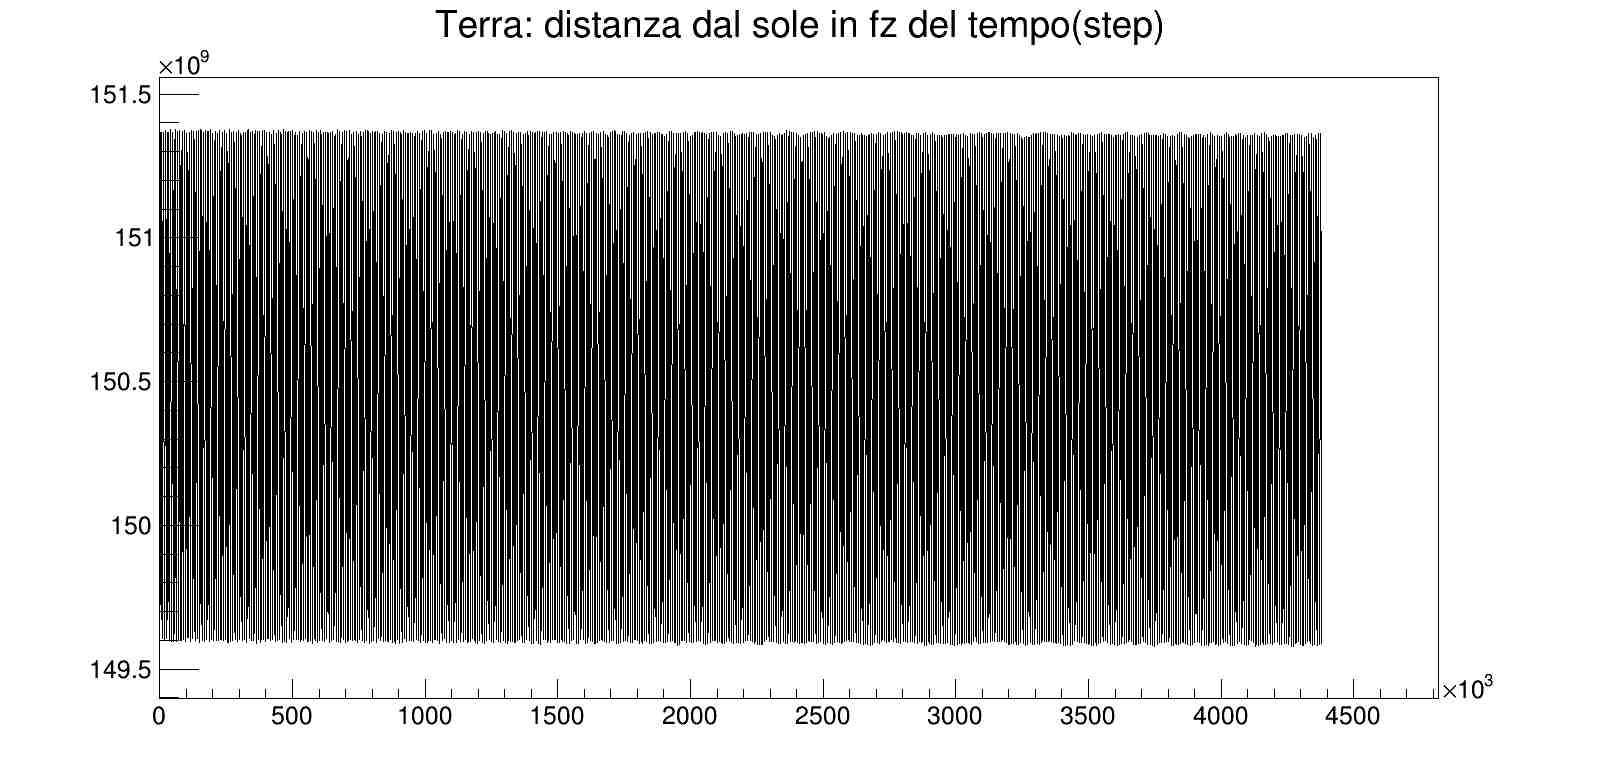
\includegraphics[width=\textwidth]{5_distanza/mototera_500.jpg}
                    \label{cfr::Terra} 
                    \caption{Dati medi(in alto) e dati mix(sotto)}
            \end{columns}
        \end{frame}
        \begin{frame}{Distanza vs T e deltaT}
            \begin{figure}
                \centering
                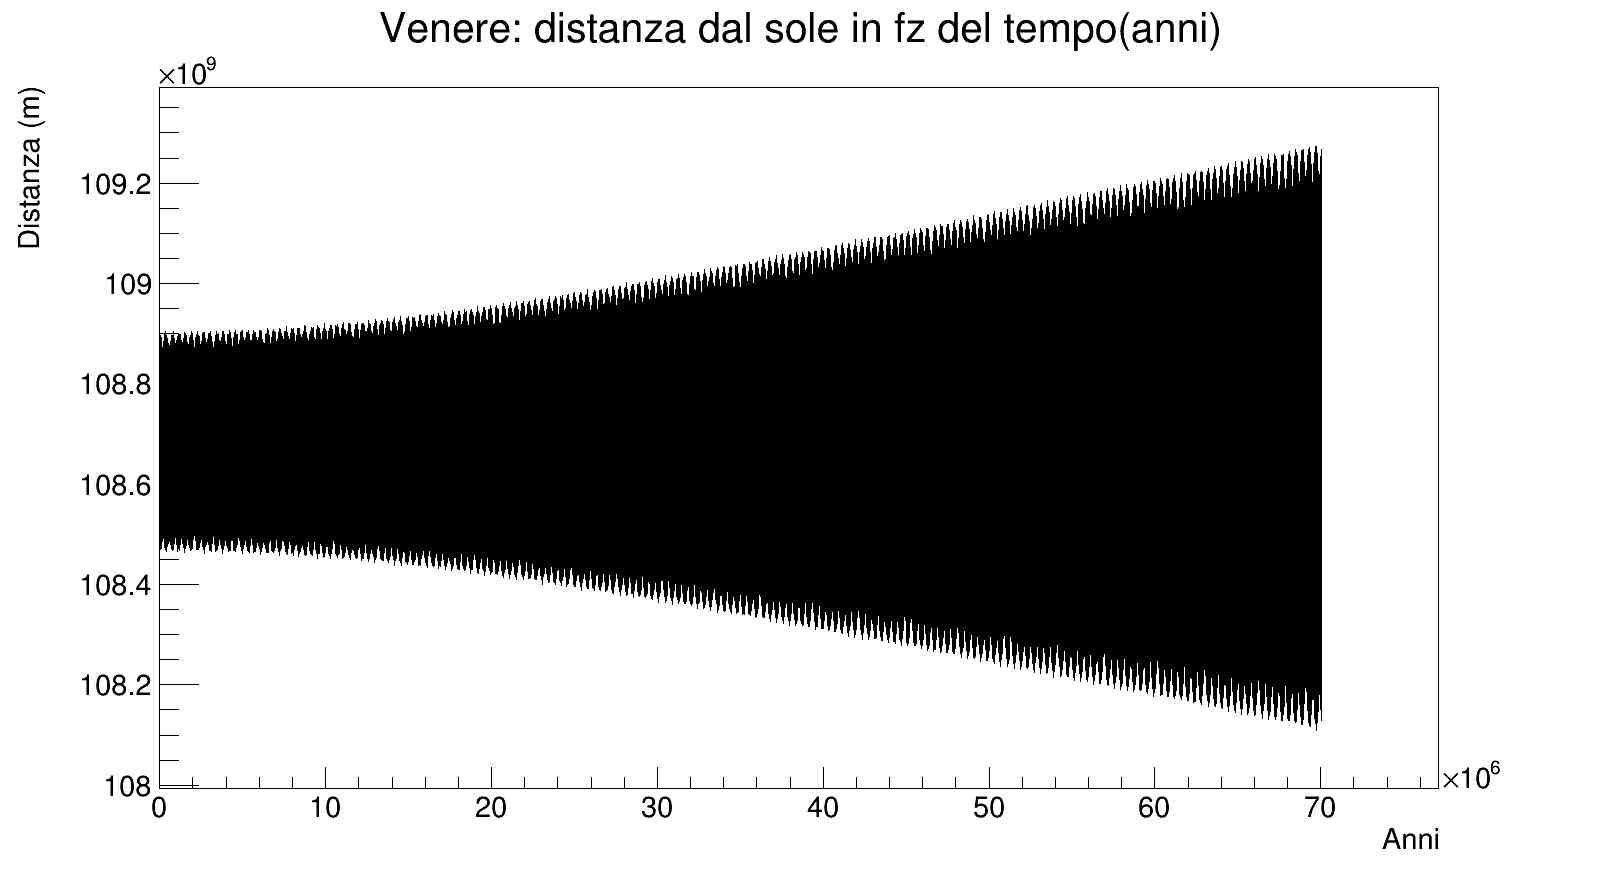
\includegraphics[width=\textwidth, height=3.75cm]{5_distanza/ven_8000_drift.jpg}\\
                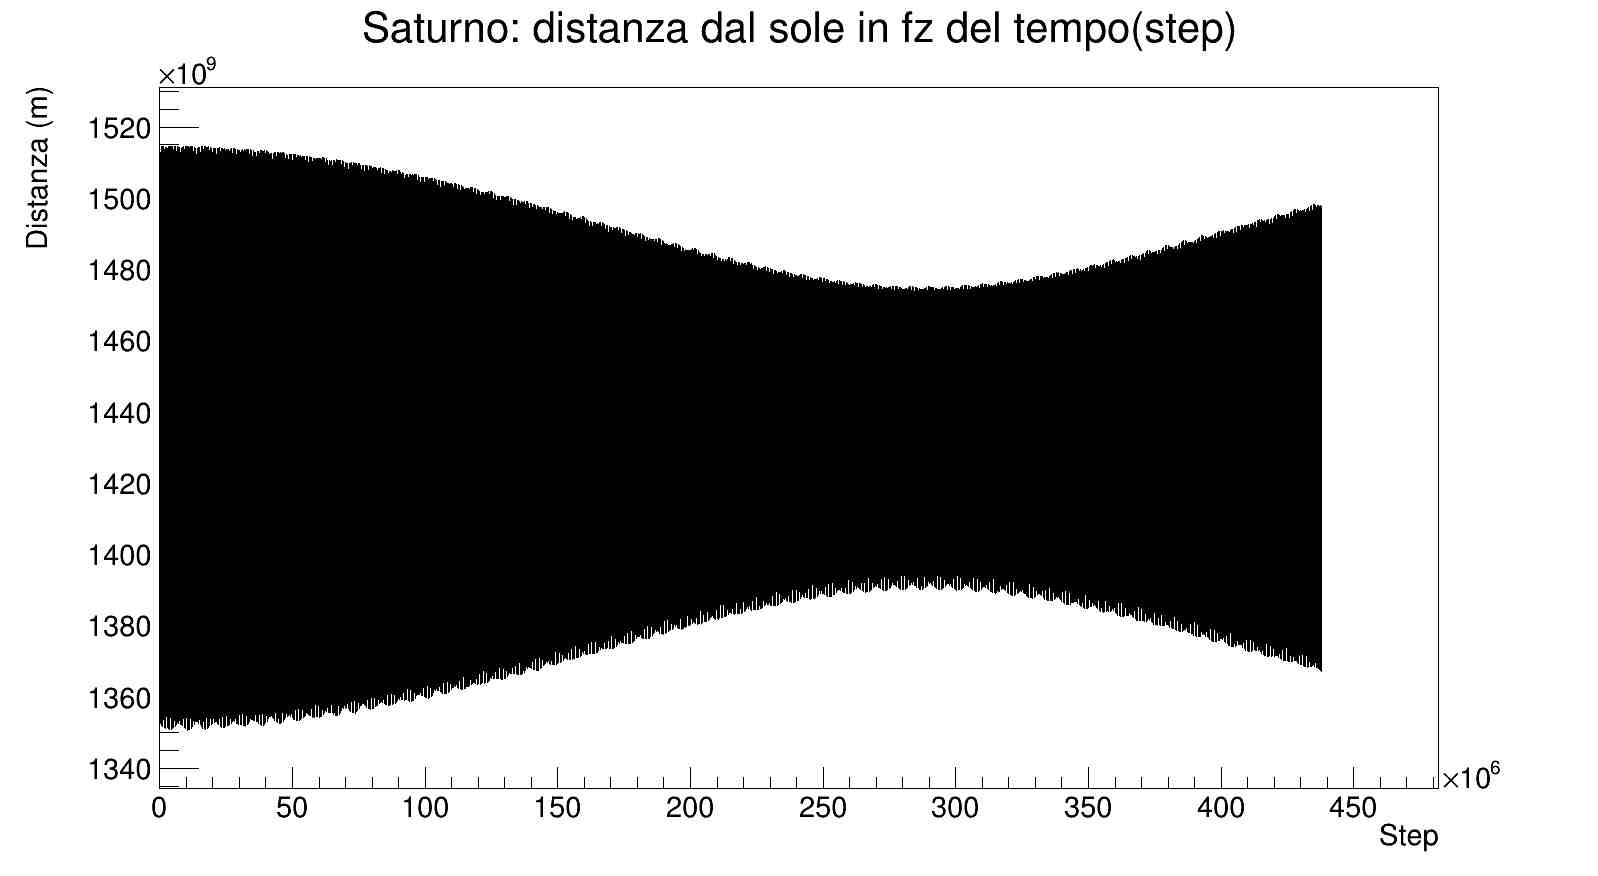
\includegraphics[width=\linewidth, height=3.75cm]{5_distanza/sat_moto_afe_bug_50k_3600.jpg}
                %\caption{Caption}
                \label{fig:8000}
            \end{figure}
        \end{frame}
        \begin{frame}{Grafici con Python}
            \begin{columns}
                \column{.5\textwidth}
                    \centering        
                    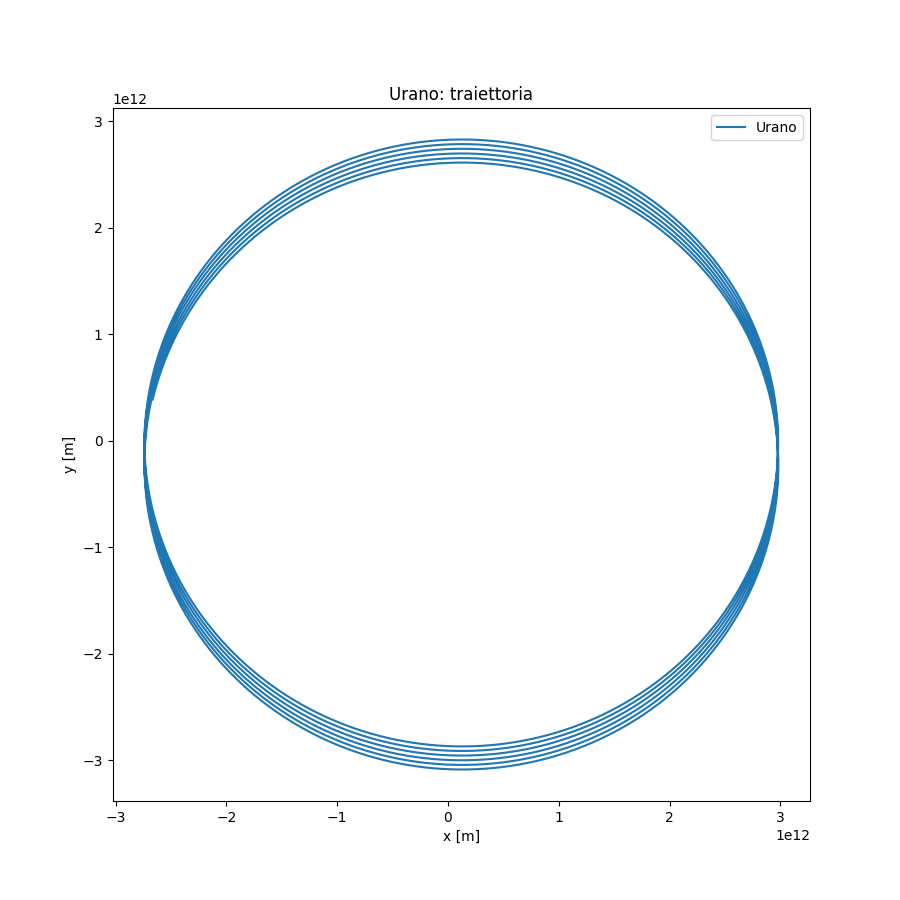
\includegraphics[width=5cm,height=5cm]{5_distanza/ura_orbita.png}      
                \column{.5\textwidth}
                    \centering        
                    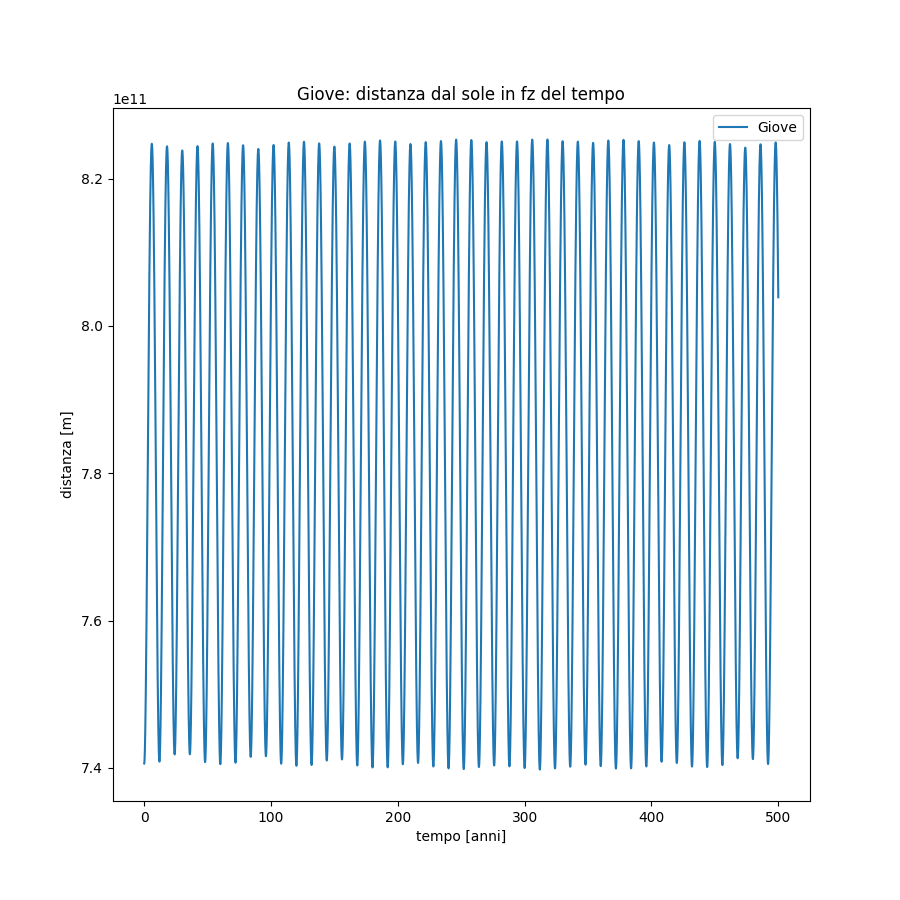
\includegraphics[width=5cm,height=3.75cm]{5_distanza/gio_osc_500_bello.png}\\
                    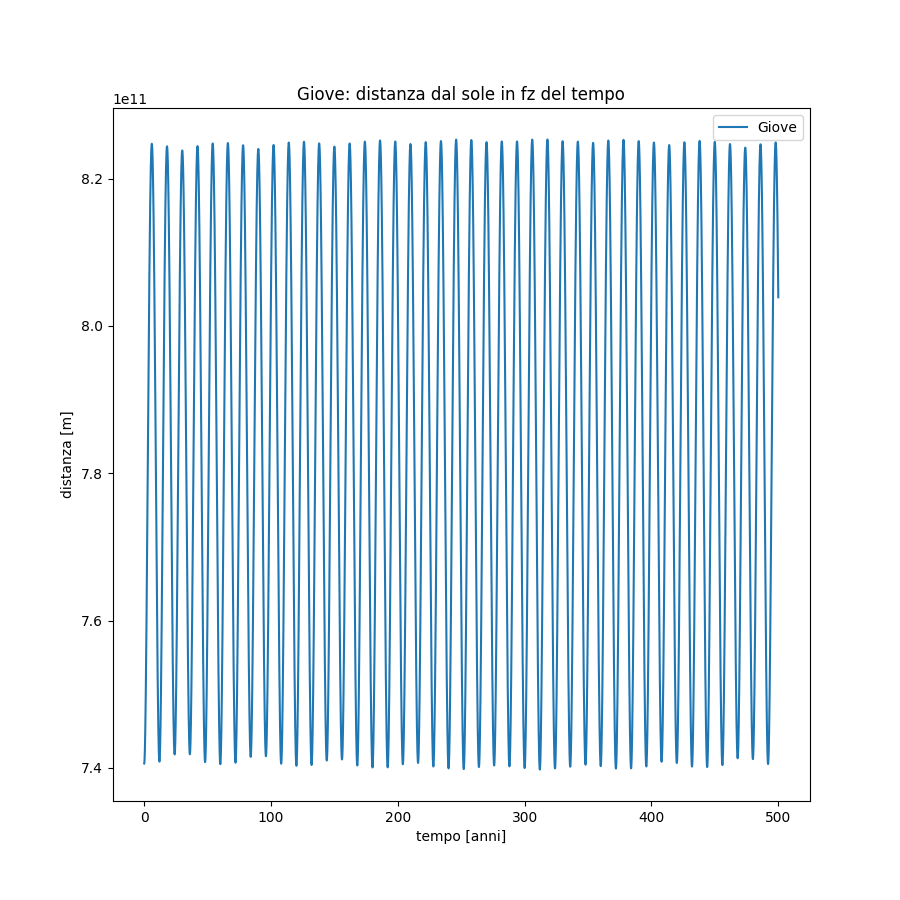
\includegraphics[width=5cm,height=3.75cm]{5_distanza/gio_osc_500_bello.png} 
            \end{columns}
        \end{frame}